\pagenumbering{arabic}
\section{决策树算法实现流程}
\subsection{什么是决策树算法}
决策树是一树状结构,它的每一个叶节点对应着一个分类,非叶节点对应着在某个属性上的划分,根据样本在该属性上的不同取值将其划分成若干个子集。对于非纯的叶节点,多数类的标号给出到达这个节点的样本所属的类。构造决策树的核心问题是在每一步如何选择适当的属性对样本做拆分。对一个分类问题,从已知类标记的训练样本中学习并构造出决策树是一个自上而下,分而治之的过程。

本节下面的内容将开始讲解决策树的具体内容。首先将从一个最经典的决策树分类算法开始说明决策树。

ID3算法基于信息熵来选择最佳测试属性。它选择当前样本集中具有最大信息增益值的属性作为测试属性;样本集的划分则依据测试属性的取值进行,测试属性有多少不同取值就将样本集划分为多少子样本集,同时决策树上相应于该样本集的节点长出新的叶子节点。ID3算法根据信息论理论,采用划分后样本集的不确定性作为衡量划分好坏的标准,用信息增益值度量不确定性:信息增益值越大,不确定性越小。因此,ID3算法在每个非叶节点选择信息增益最大的属性作为测试属性,这样可以得到当前情况下最纯的拆分,从而得到较小的决策树。

设$S$是$s$个数据样本的集合。假定类别属性有$m$个不同的值:$C_i(i=1,2,...,m)$ 。

设$s_i$是类$C_i$中的样本数。对一个给定的样本,它总的信息熵为
\begin{equation}
I(s_1,s_2,...,s_m)=a\sum_{i=1}^m P_i-\log_2(P_i)
 \end{equation}
                  
其中,$P_i$ 是任意样本属于$C_i$的概率,一般可以用$\frac{s_i}{s}$ 估计。

设一个属性A具有$k$个不同的值,$\{a_1,a_2,...,a_k\}$利用属性A将集合$S$划分为个$k$子集,$\{S_1,S_2,...,S_k\}$其中$S_j$包含了集合$S$中属性A取$a_j$值的样本。若选择属性A为测试属性,则这些子集就是从集合$S$的节点生长出来的新的叶节点。设$s_{ij}$是子集$S_j$中类别为$C_i$的样本数,则根据属性A划分样本的信息熵值为

\begin{equation}
E(A)=a\sum_{j=1}^k\frac{s_{1j}+s_{2j}+...+s_{mj}}{s}I(s_{1j},s_{2j},...,s_{mj})
\end{equation}

其中,$I(s_{1j},s_{2j},...,s_{mj})=a\sum_{i=1}^mP_{ij}-\log_2(P_{ij})$,$P_{ij}=\frac{s_{ij}}{s_{1j}+s_{2j}+...+s_{mj}}$是子集$S_j$中类别为$C_i$的样本的概率。

最后,用属性A划分样本集S后所得的信息增益(Gain)为

\begin{equation}
 Gain(A)=I(s_1,s_2,...,s_m)-E(A) 
\end{equation}

显然E(A)越小,Gain(A)的值越大,说明选择测试属性A对于分类提供的信息越大,选择A之后对分类的不确定程度越小。属性A的k个不同的值对应的样本集S的k个子集或分支,通过递归调用上述过程(不包括己经选择的属性),生成其他属性作为节点的子节点和分支来生成整个决策树。ID3决策树算法作为一个典型的决策树学习算法,其核心是在决策树的各级节点上都用信息增益作为判断标准来进行属性的选择,使得在每个非叶节点上进行测试时,都能获得最大的类别分类增益,使分类后的数据集的熵最小。这样的处理方法使得树的平均深度较小,从而有效地提高了分类效率。

ID3算法具体流程

ID3算法的具体详细实现步骤如下:

(1)对当前样本集合,计算所有属性的信息增益;

(2)选择信息增益最大的属性作为测试属性,把测试属性取值相同的样本划为同一个子样本集;

(3)若子样本集的类别属性只含有单个属性,则分支为叶子节点,判断其属性值并标上相应的符号,然后返回调用处;否则对子样本集递归调用本算法。

下面将结合餐饮案例实现ID3的具体实施步骤。T餐饮企业作为大型连锁企业,生产的产品种类比较多,另外涉及的分店所处的位置也不同,数目比较多。对于企业的高层来讲,了解周末和非周末销量是否有大的区别,以及天气、促销活动这些因素是否能够影响门店的销量这些信息至关重要。因此,为了让决策者准确了解和销量有关的一系列影响因素,需要构建模型来分析天气、是否周末和是否有促销活动对销量的影响,下面以单个门店来进行分析。

对于天气属性,数据源中存在多种不同的值,这里将那些属性值相近的值进行类别整合。如天气为“多云”、“多云转晴”、“晴”这些属性值相近,均是适宜外出的天气,不会对产品销量有太大的影响,因此将它们为一类,天气属性值设置为“好”,同理对于“雨”、“小到中雨”等天气,均是不适宜外出的天气,因此将它们为一类,天气属性值设置为“坏”。

对于是否周末属性,周末则设置为“是”,非周末则设置为“否”。

对于是否有促销活动属性,有促销则设置为“是”,无促销则设置为“否”。

产品的销售数量为数值型,需要对属性进行离散化,将销售数据划分为“高”和“低”两类。将其平均值作为分界点,大于平均值的划分到类别“高”,小于平均值的划分为“低”类别。

经过以上的处理,我们得到的数据集合如表。

\begin{table}[thbp]\footnotesize
	\caption{处理后的数据集}
	\begin{center}
		\begin{tabular}{c|c|c|c|c}
			\hline  序号& 天气 & 是否周末&是否有促销&  销量\\ 
			\hline 1 & 坏 & 是&是&高 \\ 
			\hline 2 & 坏 & 是&是&高 \\ 
			\hline 3 & 坏 & 是&是&高 \\ 
			\hline 4 & 坏 & 否&是&高 \\ 
			\hline ...& ... & ...&...&... \\ 
			\hline 32 & 好 & 否&是&低 \\ 
			\hline 33 & 好 & 否&否&低 \\ 
			\hline 34 & 好 & 否&否&低 \\ 
			\hline
		\end{tabular} 
	\end{center}
\end{table}

采用ID3算法构建决策树模型的具体步骤如下:

(1)根据公式,计算总的信息熵,其中数据中总记录数为34,而销售数量为“高”的数据有18,“低”的有16。

\begin{equation}
I(18,16)=\frac{18}{34}\log_2\frac{18}{34}-\frac{16}{34}\log_2\frac{16}{34}=0.997503
\end{equation}

(2)根据公式,计算每个测试属性的信息熵。

对于天气属性,其属性值有“好”和“坏”两种。其中天气为“好”的条件下,销售数量为“高”的记录为11,销售数量为“低”的记录为6,可表示为(11,6);天气为“坏”的条件下,销售数量为“高”的记录为7,销售数量为“低”的记录为10,可表示为(7,10)。则天气属性的信息熵计算过程如下:

\begin{equation}
I(11,6)=\frac{11}{17}\log_2\frac{11}{17}-\frac{6}{17}\log_2\frac{6}{17}=0.936667
\end{equation}

\begin{equation}
I(7,10)=\frac{7}{17}\log_2\frac{7}{17}-\frac{10}{17}\log_2\frac{10}{17}=0.977418
\end{equation}

\begin{equation}
E(\mbox{天气})=\frac{17}{34}I(11,6)+\frac{17}{34}I(7,10)=0.957043
\end{equation}

对于是否周末属性,其属性值有“是”和“否”两种。其中是否周末属性为“是”的条件下,销售数量为“高”的记录为11,销售数量为“低”的记录为3,可表示为(11,3);是否周末属性为“否”的条件下,销售数量为“高”的记录为7,销售数量为“低”的记录为13,可表示为(7,13)。则节假日属性的信息熵计算过程如下:

\begin{equation}
I(11,3)=\frac{11}{14}\log_2\frac{11}{14}-\frac{3}{14}\log_2\frac{3}{14}=0.749595
\end{equation}

\begin{equation}
I(7,13)=\frac{7}{20}\log_2\frac{7}{20}-\frac{13}{20}\log_2\frac{13}{20}=0.934068
\end{equation}

\begin{equation}
E(\mbox{是否周末})=\frac{14}{34}I(11,3)+\frac{20}{34}I(7,13)=0.858109
\end{equation}

对于是否有促销属性,其属性值有“是”和“否”两种。其中是否有促销属性为“是”的条件下,销售数量为“高”的记录为15,销售数量为“低”的记录为7,可表示为(15,7);其中是否有促销属性为“否”的条件下,销售数量为“高”的记录为3,销售数量为“低”的记录为9,可表示为(3,9)。则是否有促销属性的信息熵计算过程如下:

\begin{equation}
I(15,7)=\frac{15}{22}\log_2\frac{15}{22}-\frac{7}{22}\log_2\frac{7}{22}=0.902393
\end{equation}

\begin{equation}
I(3,9)=\frac{3}{12}\log_2\frac{3}{12}-\frac{9}{12}\log_2\frac{9}{12}=0.811278
\end{equation}

\begin{equation}
E(\mbox{是否有促销})=\frac{22}{34}I(15,7)+\frac{12}{34}I(3,9)=0.870235
\end{equation}

(3)根据公式,计算天气、是否周末和是否有促销属性的信息增益值。

$Gain(\mbox{天气})=I(18,16)-E(\mbox{天气})=0.997503-0.957043=0.04046$

$Gain(\mbox{是否周末})=I(18,16)-E(\mbox{是否周末})=0.997503-0.858109=0.139394$

$Gain(\mbox{是否有促销})=I(18,16)-E(\mbox{是否有促销})=0.997503-0.870235=0.127268$

(4)由第3步的计算结果可以知道是否周末属性的信息增益值最大,它的两个属性值“是”和“否”作为该根结点的两个分支。然后按照第1步到第3步所示步骤继续对该根结点的三个分支进行结点的划分,针对每一个分支结点继续进行信息增益的计算,如此循环反复,直到没有新的结点分支,最终构成一棵决策树。生成的决策树模型如下图:

\begin{figure}[thbp!]
	\centering
	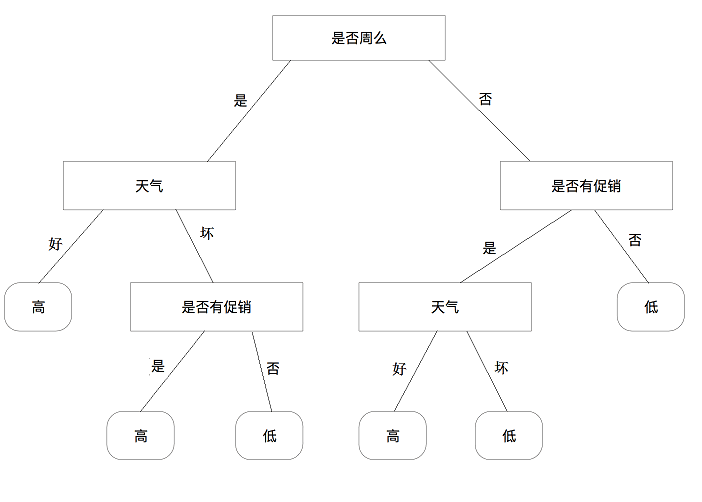
\includegraphics[width=0.4\linewidth]{figure/3-1}
	\caption{\ 全局离群点和局部离群点}
	\label{fig:3-1}
\end{figure}

从上面的决策树模型可以看出,门店的销售高低和各个属性之间的关系,并可以提取出以下决策规则:

\begin{itemize}
	\item 若周末属性为“是”,天气为“好”,则销售数量“高”;
	\item 若周末属性为“是”,天气为“坏”,促销属性为“是”,则销售数量“高”;
	\item 若周末属性为“是”,天气为“坏”,促销属性为“否”,则销售数量“低”;
	\item 若周末属性为“否”,促销属性为“否”,则销售数量“低”;
	\item 若周末属性为“否”,促销属性为“是”,天气为“好”,则销售数量“高”;
	\item 若周末属性为“否”,促销属性为“是”,天气为“坏”,则销售数量“低”;
\end{itemize}

由于ID3决策树算法采用了信息增益作为选择测试属性的标准,会偏向于选择取值较多的即所谓高度分支属性,而这类属性并不一定是最优的属性。同时ID3决策树算法只能处理离散属性,对于连续型的属性,在分类前需要对其进行离散化。为了解决倾向于选择高度分支属性的问题,人们采用信息增益率作为选择测试属性的标准,这样便得到C4.5决策树算法。此外常用的决策树算法还有CART算法、SLIQ算法、SPRINT算法和PUBLIC算法等等。

\subsection{数据决策树处理}

本文主要使用RapidMiner中的决策树算子对所给数据进行处理后分别生产两个决策树:

(1)驻地决策树:这个决策树是以文化程度为label,以驻地为展示属性来反映不同文化程度数据类构造的驻地规则。

(2)工种决策树:这个决策树是以工种为label,反映出不同工种对应的文化程度,驻地的相关性规律。
